\documentclass[a4paper,openright,12pt]{book}
\usepackage[spanish,  es-tabla]{babel}
\usepackage[utf8]{inputenc}
\usepackage{graphicx}
\usepackage{multirow, array}
\usepackage{longtable}
\usepackage{graphicx}
\usepackage{colortbl}
\usepackage{listings}

\begin{document}

\begin{titlepage}

  \begin{center}

    \vspace*{-1in}
    \begin{figure}[htb]
      \begin{center}
        
\includegraphics[width=8cm]{ciencias2}
      \end{center}
    \end{figure}

    FACULTAD DE CIENCIAS

    \vspace*{0.15in}

    DEPARTAMENTO DE MATEMATICAS

    \vspace*{0.6in}

    \begin{large}
      EXPERIENCIA PROFESIONAL
    \end{large}

    \vspace*{0.2in}

    \begin{Large}
      \textbf{Implementación de un nuevo modelo de consulta de información y
        reestructura de arquitectura de datos}
    \end{Large}

    \vspace*{0.3in}

    \begin{large}
      Trabajo por experiencia profesional presentado por Erick Celso Zavaleta
      González para obtener el grado de Licenciado en Ciencias de la Computación
    \end{large}

    \vspace*{0.3in}
    \rule{80mm}{0.1mm}
    \vspace*{0.1in}

    \begin{large}
      Supervisados por: Dr. Canek Peláez Valdés
    \end{large}

  \end{center}

\end{titlepage}

\newpage
$\ $
 % para que no se numere esta pagina
\thispagestyle{empty}

\chapter*{}
% para comenzar la numeracion de paginas en numeros romanos
\pagenumbering{Roman}
\begin{flushright}
\textit{Dedicado a... }
\end{flushright}

% si no queremos que añada la palabra ``Capitulo''
\chapter*{Agradecimientos}
% si queremos que aparezca en el índice
\addcontentsline{toc}{chapter}{Agradecimientos}
% encabezado
\markboth{AGRADECIMIENTOS}{AGRADECIMIENTOS}

¡Muchas gracias a todos!

% indice de contenidos
\tableofcontents

\cleardoublepage
% para que aparezca en el indice de contenidos
\addcontentsline{toc}{chapter}{Lista de figuras}
% indice de figuras
\listoffigures

\cleardoublepage
% para que aparezca en el indice de contenidos
\addcontentsline{toc}{chapter}{Lista de tablas}
% indice de tablas
\listoftables

% si no queremos que añada la palabra ``Capitulo''
\chapter*{Marco Teórico}
\label{cap.mteorico}
\pagenumbering{arabic}
% si queremos que aparezca en el índice
\addcontentsline{toc}{section}{Marco Teórico}
% encabezado
\markboth{Marco Teórico}{Marco Teórico}

El marco teórico del proyecto se basa en laarquitecura de datos, que en
tecnología de la información se compone de los modelos, políticas, reglas y/o
estándares que determinan qué datos se recolectan y cómo se guardan, ordenan,
integran y usan en los sistemas de datos de una institución.

Hablar de datos es entrar en un mundo complejo donde existen diferentes
perspectivas de datos, dependiendo del uso que se les quiera dar o de las
personas que lo utilizan. Cada grupo de personas tiene su propia perspectiva
sobre el manejo de datos: manejo de grandes volúmenes, acceso al detalle de los
datos de manera instantánea, manejo de la integridad, datos de acceso exclusivo,
etc. La arquitectura de datos nos ayuda a que estos diferentes tipos de datos y
diferentes necesidades puedan coexistir de una forma conjunta de acuerdo a las
necesidades de cada área o empresa.

Actualmente no existe ningún secreto para el manejo de datos y su respectiva
arquitectura; en ambos casos, es importante entender los datos en términos de su
infraestructura; es decir, se requiere conocer la infraestructura que rodea a
los datos para llevar a cabo un uso adecuado de los mismos.

Así mismo, es importante saber que dentro de cualquier empresa u organización se
pueden encontrar diferentes tipos de datos: estructurados y no
estructurados. Los primeros son datos predecibles y que normalmente son
manejados en una base de datos (SMBD): registros, atributos, llaves, índices,
etc. Por su parte, los datos no estructurados no son predecibles y, como su
nombre lo indica, no tienen una estructura bien definida, usualmente son de
dificil acceso y generalmente se requiere una búsqueda más profunda para hacer
consultas; por ejemplo, una cadena de carácteres en un texto libre.

Todos estos conceptos serán detallados y aplicados en los capítulos del proyecto
presentado.

% si no queremos que añada la palabra ``Capitulo''
\chapter*{Objetivo y Justificación}
\label{cap.objetivo}
% si queremos que aparezca en el índice
\addcontentsline{toc}{section}{Objetivo y Justificación}
% encabezado
\markboth{Objetivo y Justificación}{Objetivo y Justificación}

El proyecto que se presenta fue la implementación y reestructura de la
infraestructura de base de datos, así como los cambios en procesos y
arquitectura de datos de una institución financiera que por razones de acuerdos
de confidencialidad no puedo mencionar su nombre. Dentro de las actividades que
realicé se encuentra un análisis del software a utilizar, así como la definición
y desarrollo de programas para convertir los datos de diferentes bases de datos
y plataformas hacia un repositorio de datos único que ayudó a eficientar los
tiempos de respuesta y las consultas realizadas.

Las bases en desarrollo de software, bases de datos, estructuras de datos,
lenguajes de programación y, por encima de todo, análisis y solución de
problemas que obtuve dentro de la carrera de Ciencias de la Computación, me
ayudarón a que dicho proyecto se realizara de manera éxitosa.

% si no queremos que añada la palabra ``Capitulo''
\chapter{Análisis de requerimientos}
\label{cap.analisis}
% si queremos que aparezca en el índice
\addcontentsline{toc}{section}{Análisis de requerimientos}
 % encabezado
\markboth{Análisis de requerimientos}{Análisis de requerimientos}

\section{Proceso de selección de software}

Parte importante para llegar a la solución propuesta fue la selección del
software en el cual se desarrolló el nuevo proceso ETL \footnote{Extracción,
  Transformación y Carga (\emph{load} en Inglés).}. La selección de software
requirió de varios pasos previos a la toma de la decisión. El proceso de
selección de software de acuerdo a la metodología de Accenture fue la siguiente:

\begin{enumerate}
\item Establecer los requerimientos de negocio.
\item Establecer los requerimientos de evaluación de las herramientas de ETL.
\item Generar una lista larga de proveedores.
\item Generar una lista corta (generalmente 3 o 4 prveedores) de candidatos.
\item Realizar  un RFP (Request For  Approval) para evaluar a  los candidatos de
  manera individual y detallada.
\item Realizar la recomendación final del producto.
\end{enumerate}

Este proceso se datalla en la figura~\ref{fig:proceso}:

\begin{figure}[htb]
  \begin{center}
    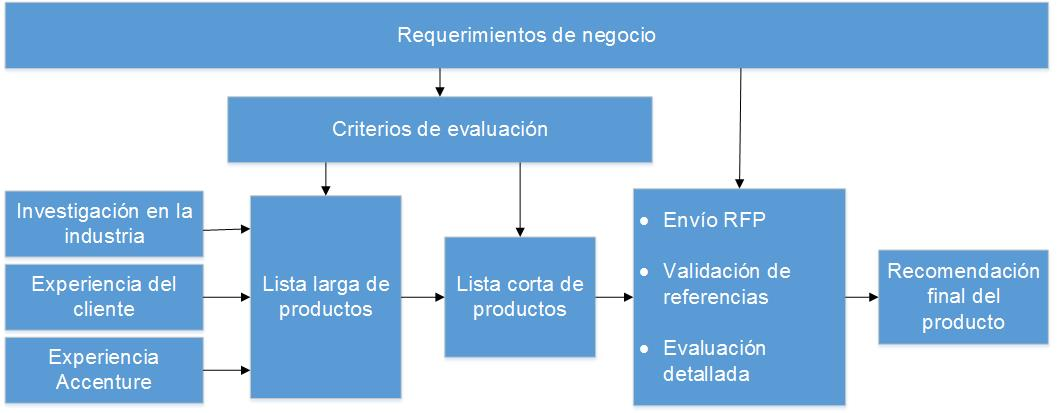
\includegraphics[width=12cm, height=3cm, scale=0.5]{Proceso_seleccion_software.jpg}
    \caption{Proceso de selección de software}
    \label{fig:proceso}
  \end{center}
\end{figure}

En las siguientes secciones se definirán cada uno de los pasos del proceso
seguidos.

\subsection{Requerimientos funcionales}

Con base en las reuniones realizadas con el área de desarrollo de sistemas de la
institución financiera se identificaron una serie de requerimientos funcionales
detallados a continuación.

\begin{itemize}

\item Se requería una conexión a correo electrónico mediante le protocolo SMTP
  para envío de informes de termino de procesos o de error en los mismos.

\item Tener un log de procesos que tuviera la información de cada uno de los
  procesos de extraccón/carga (inicio, fin, estatus de termino, errores (en cso
  de haberlos)).

\item La herramienta debía de tener la capacidad de contar con un esquema de
  limpieza de datos que permitiera identificar y corregir los errores en
  nombres, direcciones, RFC's, números de teléfono, y algunos otros datos
  relevantes para la institución financiera.

\item Permitir invocar a la herramienta ETL desde otras aplicaciones tales como
  PeopleSoft, aplicaciones desarrolladas en Java y .NET.

\item Permitir control y detalle de los errores presentados en los procesos o en
  cada uno de los componentes del flujo de datos. El control se llevaría a cabo
  mediante el envío, por parte del ETL, de errores a tablas log o archivos de
  texto en dode se pudieran identificar de una manera sencilla, los errores
  presentados.

\item Contar con un esquema de datos redundante, como puede ser un cluster,
  bases de datos replicadas, balanceo de cargas con tolerancia a fallos, etc.

\item Contar con un esquema de control de versiones que soporte el trabajo de
  multiples usuarios al mismo tiempo.

\item La herramienta debía tener la capacidad para entregar diferentes archivos
  a los sistemas destino (archivos de texto, tablas en base de datos, XML, PDF,
  Excel).

\item Contar con un esquema de seguridad basado en roles y jerarquías de usuario
  que permitieran a los usuarios acceder a datos específicos de la base de datos
  de acuerdo a su rol.

\item Contar con pantallas de configuración que permitieran a los
  administradores de la herramienta tener un mayor control sobre los procesos y
  los usuarios. Así mismo, que fuera una herramienta visualmente fácil de usar.

\item Permitir a la nueva herramienta la convivencia con las tecnologías con las
  que contaba la institución financiera (Windows 2003, SQL Server 2005, Oracle,
  DB2, AS400, Windows Vista y Mainframes)

\item Contar con una herramienta de fácil manejo de metadatos.

\item Contar con un ambiente de diseño y desarrollo 100\% visual que permitiera
  a los desarrolladores implementar las soluciones de extracción y carga de una
  manera sencilla.

\item Permitir la operación y administración de la herramienta de una forma
  remota.

\item Generar componentes reutilizables entre aplicaciones y entre procesos.

\item La herramienta debía permitir a los usuarios, la creación de funciones
  personalizadas que cumplieran con los estándares de la empresa y que no fueran
  parte de las configuraciones predefinidas de la herramienta.

\item Capacidad para calendarizar procesos; es decir, la herramienta debería ser
  capaz de ejecutar los procesos de forma automática a la hora y día
  especificados.

\item Soportar modelos de minería de datos que ayudarían a la institución
  financiera a realizar un anaálisis de sus datos y poder definir estrategias de
  mercado para los diferentes productos que ofecían.

\item Capacidades de soporte para DataWarehouse y Business Intelligence, este
  requerimiento era para cumplir con el plan estratégico de la institución.

\item Capacidad de la herramienta para plublicar procesos como Web Services a
  fin de poder acceder a ellos de manera remota o ejecutarlos a través de un
  portal con los permisos correspondientes.

\item Capacidades de detección y correción de errores en los procesos, mediante
  un proceso de depuración (Debugging) que sería ejecutado paso a paso.

\item Como un requerimiento básico, la herramienta debería de almacenar la
  información extraída en una sola fuente de datos, para la solución propuesta
  fue una base de datos de paso llamada base de datos stage.

\item Explotación de la información de una base centralizada para realizar
  reportes.

\item Consulta de datos históricos, en especial de transacciones, para poder ser
  explotados desde otro ambiente o aplicación existente en la institución
  financiera.

\item La herramienta debería de ser capaz de obtener solamente la información
  que tuvo cambios entre los diferentes periodos de extracción, ayudando al
  rendimiento del proceso y extrayendo una cantidad menor de datos.
\end{itemize}

\subsection{Requerimientos técnicos}

Por su parte los requerimientos técnicos solicitados por la institución para
seleccionar la herramienta fueron los siguientes:

\begin{itemize}

\item Mejorar el rendimiento de la extracción de datos de 90 minutos a 45
  minutos (tiempo tentativo) con una cantidad de 6 millones de registros

\item Mejorar el tiempo de transformación de datos utilizando componentes para
  limpieza y calidad de los datos.

\item Mejorar el rendimiento de la herramienta cuando el volumen de datos exceda
  los 100 millones de registros.

\item Que la arquitectura de la herramienta fuera compatible con la arquitectura
  de la institución y la futura que se planteó en el presente proyecto.

\item La herramienta debía ser capaz de poder integrarse son los sistemas de la
  institución (PeopleSoft, Core bancario, systema de reportes, sistema de
  recursos humanos, pagos a terceros, etc.)

\item La herramienta debía ser capaz de ejecutarse en diferentes paltaformas
  (Windows, Linux, Unix, Mainframes).

\item Conectividad con los istemas fuentes (ODBC, OLAP, LDAP) y con diferentes
  sistemas manejadores de bases de datos como Oracle, DB2, SQL Server, Informix,
  Sybase, Teradata.

\item Capacidad para crear funciones y métodos desde cualquier lenguaje de
  programación estructurado y que pudiera ser ejecutado desde la herramienta
  ETL.
\end{itemize}

Aunque el gobierno de datos no era parte del alcance del proyecto, pero si de la
estrategia de crecimiento de la institución, la herramienta debería de soportar
esta funcionalidad.

\subsection{Requerimientos de limpieza de datos}

Como parte de la definición de requerimientos funcionales que debía cumplir la
herramienta, existe una sección que tenía que ver con la calidad y limpieza de
datos; estos requerimientos solicitados por parte del área de tecnoloía fueron
los siguientes:

Se requería que el proceso ETL realizara la limpieza de datos de los campos
descritos a continuación:

\begin{itemize}

\item RFC. Se requería que el RFC se encontrara estandarizado y cumplieran con
  los requerimientos establecidos por el buró de crédito

\item Nombres de socios. Se requería que los nombres de socios no tuvieran
  caracteres especiales como puntos, comas, retornos de carro, paréntesis,
  corchetes, porcentaje, comillas y caracteres de 16 bits.

\item Fechas de morosidad. Se solicitó que las fechas para el cálculo de la
  morosidad se encontraran en un formato de fecha correcto yyyymmdd y que no se
  permitieran valores nulos o negativos para este tipo de dato.

\item Direcciones de socios. Fue requerido que las direcciones de los socios
  tuvieran una nomenclatura estándar para nombres de calles, colonias

\item Ciudades/Municipios. Los códigos y nombres de ciudades y municipios debían
  de contar con un estándar y estos deberian de estar corregidos de a cuerdo a
  la información proporcionada por SEPOMEX.

\item Teléfonos. Los teléfonos de los clientes debían contar con la clave lada y
  todos tenían que ser de 10 dígitos para números fijos y de 13 dígitos para
  números celulares

\item Los números telefónicos no deberían de tener guiones o caracteres
  especiales.
\end{itemize}

Como parte de la estandarización de direcciones era requerido que todos los
códigos postales se encontraran conforme a la lista proporcionada por SEPOMEX y
todos deberían de ser de 5 dígitos.

\section{Criterios de evaluación}

Como mencionamos al inicio del documento, parte importante de la selección de sofware fue la definición de los criterios de evaluación de la herramienta ETL a utilizar como parte del proyecto. Dichos criterios nos ayudaron a realizar una evaluación objetiva de las diferentes herramientas y tener un panorama general de los productos que cumplían con las caracteristicas y necesidades de la institución financiera. Tomando como base esas necesidades y la experiencia de Accenture se definieron los criterios de selección de software.

Los criterios se agruparon en conceptos genericos que describen la funcionalidad
de cada área. Estos criterios se listan a continuación:

\begin{enumerate}
\item \textit{Capacidades del servicio.}
\item \textit{Opciones de integración.}
\item \textit{Ambiente de la herramienta.}
\item \textit{Soporte y capacitación.}
\item \textit{Técnicas adicionales de integración de datos.}
\item \textit{Manejo de la información.}
\item \textit{Estrategias del producto.}
\item \textit{Estrategias corporativas.}
\item \textit{Costos.}
\item \textit{Convenios con otros proveedores.}
\item \textit{Finanzas de la compañia.}
\end{enumerate}

\subsection{Lista de proveedores}

Una vez que se definieron los criterios de evaluación y se realizó el análisis
de requerimientos con el equipo de la institución financiera, el siguiente paso
fue dar una lista larga de proveedores candidatos para ser evaluados y que en
ese momento eran las mejores opciones dentro del mercado. La lista contenía a 6
proveedores de software: Oracle (Oracle Warehouse Builder), Informática (Power
Center), IBM (Infosphere Information Server), Microsoft (Integration Services
(SSIS), SAP (SAP-Business Objects), SAS Institute (SAS).

\subsection{Evaluación de proveedores}

Con la lista larga de proveedores definida, la siguiente tarea que se llevó a
cabo fue la evaluación de cada uno de los proveedores con el fin de establecer
un grupo reducido de candidatos que representaría la lista final de selección de
la herramienta ETL a utilizar dentro del proyecto. De acuerdo a las necesidades
de la Institución financiera se definieron los siguientes porcentajes para los
criterios de evaluación

\begin{table}[htbp]
  \begin{center}
    \begin{tabular}{|p{6cm}|>{\centering\arraybackslash}m{3cm}|c|}
      \hline
      Criterio & Porcentaje de evaluación & Prioridad\\
      \hline
      Capacidades del servicio & 14\% & 1 \\
      \hline
      Manejo de la información & 14\% & 2\\
      \hline
      Opciones de integración & 11\% & 3\\
      \hline
      Ambiente de la herramienta & 11\% & 4\\
      \hline
      Costos & 11\% & 5\\
      \hline
      Soporte y capacitación & 9\% & 6\\
      \hline
      Estrategias del producto & 6\% & 7\\
      \hline
      Convenios con otros proveedores & 6\% & 8\\
      \hline
      Técnicas adicionales de integración de datos & 6\% & 9\\
      \hline
      Estrategias corporativas & 6\% & 10\\
      \hline
      Finanzas de la compañia proveedora & 6\% & 11\\
      \hline
    \end{tabular}
    \caption{Porcentajes y prioridades de evaluación.}
    \label{tabla:criterios}
  \end{center}
\end{table}

La prioridad de cada uno de los criterios de evaluación se realizó con base en
las necesidades de la institución y basados también en la funcionalidad de cada
uno de ellos.

Con toda la información que se recolectó, realicé un análisis de cada proveedor
y su herramientas presentadas, así como sus factores diferenciales y las
características principales soportadas. Esta evaluación se presenta en la
siguiente tabla con los resultados finales:

\begin{table}[htbp]
  \begin{center}
    \scalebox{0.75}[0.65]{
      \begin{tabular}{|p{5.5cm}|>{\centering\arraybackslash}m{1.7cm}|c|c|c|c|c|c|}
        \hline
        & & \rotatebox{90}{Microsoft SSIS}
        & \rotatebox{90}{Oracle OWB}
        & \rotatebox{90}{Informática Power center}
        & \rotatebox{90}{IBM IIS}
        & \rotatebox{90}{SAP\-Business Objects}
        & \rotatebox{90}{SAS} \\
        \hline
        & Porcentaje&&&&&&\\
        \hline
        \rowcolor[gray]{0.9}\textbf{Capacidades del servicio}
        & \textbf{14.29\%}
        & \textbf{3}
        & \textbf{3.5}
        & \textbf{4.5}
        & \textbf{4}
        & \textbf{3.75}
        & \textbf{4} \\
        \hline
        \rightline{Escalabilidad y rendimiento} & & 4 & 4 & 5 & 5 & 4 & 4 \\
        \hline
        \hspace{0.5cm}Alta disponibilidad & & 4 & 3 & 4 & 4 & 4 & 3 \\
        \hline
        \rightline{Seguridad} & & 3 & 4 & 5 & 3 & 4 & 5 \\
        \hline
        \hspace{0.5cm}Plataformas de ejecución soportadas
        & & 1 & 3 & 4 & 4 & 3 & 4 \\
        \hline
        \rowcolor[gray]{0.9}\textbf{Opciones de integración}
        & \textbf{11.43\%}
        & \textbf{3}
        & \textbf{3}
        & \textbf{4}
        & \textbf{4}
        & \textbf{3.4}
        & \textbf{3.6}\\
        \hline
        Conectividad con sistemas fuente & & 4 & 3 & 5 & 5 & 5 & 5\\
        \hline
        Conectividad para la carga & & 4 & 3 & 5 & 5 & 5 & 5\\
        \hline
        Servicios Web & & 4 & 4 & 5 & 5 & 3 & 3\\
        \hline
        Conexión a correo electrónico & & 1 & 1 & 1 & 1 & 0 & 1\\
        \hline
        Reusabilidad & & 2 & 4 & 4 & 4 & 4 & 4 \\
        \hline
        \rowcolor[gray]{0.9}\textbf{Ambientes de la herramienta}
        & \textbf{11.43\%}
        & \textbf{3.2}
        & \textbf{4}
        & \textbf{4.4}
        & \textbf{4.2}
        & \textbf{4.4}
        & \textbf{3.6} \\
        \hline
        Visualización del ambiente de diseño y desarrollo
        & & 4 & 4 & 4 & 4 & 4 & 4 \\
        \hline
        Manejo de errores & & 4 & 4 & 5 & 4 & 5 & 4\\
        \hline
        Ambiente de colaboración & & 2 & 4 & 4 & 4 & 4 & 3\\
        \hline
        Manejo y modelado de datos y metadatos & & 2 & 4 & 4 & 4 & 4 & 4 \\
        \hline
        Administración & & 4 & 4 & 5 & 5 & 5 & 3\\
        \hline
        \rowcolor[gray]{0.9}\textbf{Soporte y capacitación}
        & \textbf{8.57\%}
        & \textbf{4.25}
        & \textbf{4.75}
        & \textbf{4.25}
        & \textbf{4.5}
        & \textbf{3.75}
        & \textbf{4.75}\\
        \hline
        Soporte & & 4 & 5 & 5 & 5 & 5 & 4 \\
        \hline
        Capacitación & & 4 & 5 & 3 & 5 & 3 & 5 \\
        \hline
        Documentación & & 4 & 4 & 5 & 5 & 3 & 5 \\
        \hline
        Soporte a diferentes lenguajes & & 5 & 5 & 4 & 3 & 4 & 5 \\
        \hline
        \rowcolor[gray]{0.9}\textbf{Técnicas adicionales de integración de
        datos}
        & \textbf{5.71\%}
        &\textbf{ 4}
        & \textbf{2.5}
        & \textbf{4}
        & \textbf{3.5}
        & \textbf{3.5} & \textbf{1} \\
        \hline
        EII & & 3 & 3 & 4 & 4 & 3 & 0 \\
        \hline
        Cambio en la captura de datos & & 5 & 2 & 4 & 3 & 4 & 2 \\
        \hline
        \rowcolor[gray]{0.9}\textbf{Manejo de la información}
        & \textbf{14.29\%}
        & \textbf{3.6}
        & \textbf{3.8}
        & \textbf{4.4}
        & \textbf{4}
        & \textbf{3.4}
        & \textbf{3.2} \\
        \hline
        Reglas de transformación & & 3 & 3 & 4 & 4 & 3 & 3 \\
        \hline
        Perfiles de datos & & 5 & 5 & 4 & 5 & 4 & 4 \\
        \hline
        Calidad de datos & & 4 & 3 & 4 & 5 & 4 & 4 \\
        \hline
        Visualización de datos & & 2 & 4 & 5 & 2 & 4 & 4 \\
        \hline
        Contenido no estructurado & & 4 & 4 & 5 & 4 & 2 & 1 \\
        \hline
        \rowcolor[gray]{0.9}\textbf{Estrategias de producto}
        & \textbf{5.71\%}
        & \textbf{4}
        & \textbf{4}
        & \textbf{4}
        & \textbf{5}
        & \textbf{5}
        & \textbf{3}\\
        \hline
        \rowcolor[gray]{0.9}\textbf{strategias corporativas}
        & \textbf{5.71\%}
        & \textbf{3}
        &\textbf{ 3}
        & \textbf{4}
        & \textbf{3.5}
        & \textbf{3}
        & \textbf{3}\\
        \hline
        Contibución del producto & & 3 & 3 & 5 & 3 & 3 & 3 \\
        \hline
        Porcentaje de ganancias & & 3 & 3 & 3 & 4 & 3 & 3 \\
        \hline
        \rowcolor[gray]{0.9}\textbf{Costos}
        & \textbf{11.43\%}
        & \textbf{4.2}
        & \textbf{3.8}
        & \textbf{2.4}
        & \textbf{2.4}
        & \textbf{3.2}
        & \textbf{2.4}\\
        \hline
        Promedio del percio de venta & & 5 & 5 & 1 & 1 & 2 & 2 \\
        \hline
        Estructura de precios & & 3 & 3 & 1 & 1 & 3 & 1 \\
        \hline
        Modularidad de precios & & 5 & 5 & 5 & 5 & 5 & 5 \\
        \hline
        Pruebas de concepto & & 3 & 3 & 3 & 3 & 3 & 3 \\
        \hline
        Esquema de licenciamiento & & 5 & 3 & 2 & 2 & 3 & 1 \\
        \hline
        \rowcolor[gray]{0.9}\textbf{Convenios con otros proveedores}
        & \textbf{5.71\%}
        & \textbf{2.66}
        & \textbf{3.33}
        & \textbf{3.33}
        & \textbf{4.33}
        & \textbf{2.66}
        & \textbf{1.66}\\
        \hline
        Licenciamiento de terceros & & 1 & 2 & 4 & 5 & 2 & 1 \\
        \hline
        Venta del producto por terceros & & 5 & 3 & 3 & 3 & 3 & 2 \\
        \hline
        Integradores de sistemas & & 2 & 5 & 3 & 5 & 3 & 2 \\
        \hline
        \rowcolor[gray]{0.9}\textbf{Finanzas de la compañia}
        & \textbf{5.71\%}
        & \textbf{4}
        & \textbf{3}
        & \textbf{4.66}
        & \textbf{4.33}
        & \textbf{4.33}
        & \textbf{5}\\
        \hline
        Ganancias & & 3 & 2 & 5 & 5 & 3 & 5 \\
        \hline
        Crecimiento de ganancias & & 4 & 2 & 4 & 3 & 5 & 5 \\
        \hline
        Estatus del procveedor & & 5 & 5 & 5 & 5 & 5 & 5 \\
        \hline
        Total
        & 100.00\% & 168.91 & 171.18 & 190.45 & 186.76 & 172.65 & 158.21 \\
        \hline
        \rowcolor[gray]{0.9}\textbf{Calificación total}
        & & \textbf{3.54}
        & \textbf{3.52}
        & \textbf{4.0}
        & \textbf{3.98}
        & \textbf{3.67}
        & \textbf{3.20} \\
        \hline
      \end{tabular}}
    \caption{Porcentajes y prioridades de evaluación.}
    \label{tabla:criterios}
  \end{center}
\end{table}

\section{Lista corta de proveedores}

Con base en los criterios de selección y al análisis de las capacidades de cada
una de las herramientas, se obtuvo la lista corta de los proveedores. Los
proveedores seleccionados fueron los siguientes:

\begin{itemize}
\item IBM
\item Informática
\item Oracle
\item Microsoft
\end{itemize}

Si bien SAP-Business objects tenía una calificación mayor, el negocio decidió no
incluirlo en la lista final debido a que no se contaba con capacitación
suficiente de parte del proveedor. Así mismo, Microsoft se incluyó a petición
explicita de la institución.

La recomendación proporcionada por Accenture fue Informática debido a que al ser
una empres independiente enfocada a la integración de datos, no estaba casado
con ninguna base de datos específica, como si lo están el resto de los
participantes , y esto permitiría una mejor integración a las necesidades de la
institución. Basados en esta recomendación la institución financiera se decidió
por esta solución para implementar sus nuevos procesos ETL.


\section{Análisis de fortalezas y debilidades}

\section{Definición de los requerimientos}

% si no queremos que añada la palabra ``Capitulo''
\chapter*{Diseño funcional y técnico}
% si queremos que aparezca en el índice
\label{cap.diseno}
\addcontentsline{toc}{section}{Diseño funcional y técnico}
% encabezado
\markboth{Dise\~o funcional y técnico}{Diseño funcional y técnico}

\section{Arquitectura de aplicaciones (alto nivel)}

La arquitectura definida para las aplicaciones destino y fuente que se
consideraron dentro del alcance del proyecto se muestran en la siguiente figura;
dentro de esta arquitectura de aplicaciones se consideró el proceso ETL que se
construyó.

\begin{figure}[htb]
  \begin{center}
    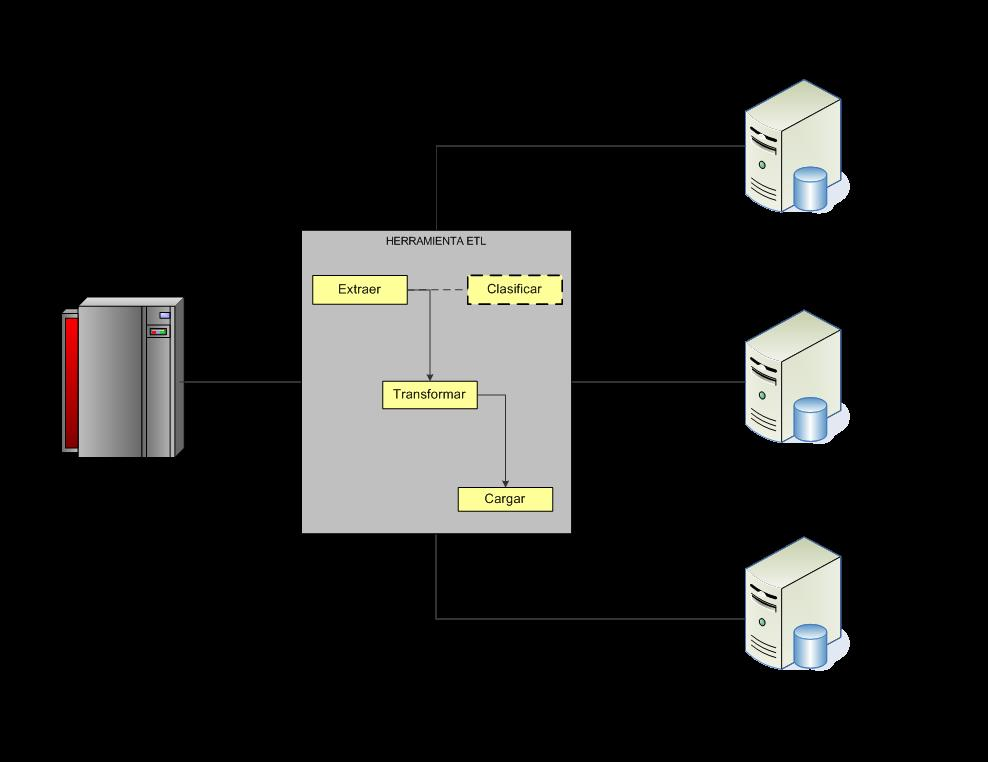
\includegraphics[width=12cm, height=3cm, scale=0.5]{Arquitectura.jpg}
        \caption{Arquitectura de aplicaciones.}
    \label{fig:arquitectura}
  \end{center}
\end{figure}

La arquitectura definida contenía al core bancario como sistema fuente de
información y enviaba la información a la herramienta ETL seleccionada para
realizar los procesos de extracción, transformación, clasificación y carga hacia
los sistemas destino y hacia cada uno de los tipos de datos que necesitaban los
equipos y bases de datos destino.


\section{Arquitectura de aplicaciones (arquitectura detallada)}

La arquitectura diseñada se encontraba dividida en cuatro capas y representan el
flujo de información entre cada una de dichas capas. La capa de interfaz de
usuario donde se realizaron todas las tareas de monitoreo, manejo de la
herramienta y visualización de datos en el sistema destino. La capa de
presentación únicamente contenía el servidor de correo que envía la información
a la capa de interfaz de usuario. Por su parte la capa de integración contenía
los procesos de la herramienta ETL; así como la base de datos stage y la base de
datos de catálogos; esta capa también incluía a las aplicaciones que envíaban
información complementaria a los sistemas destino. Finalmente contabamos con la
capa de datos que contenía a los sistemas destino, el sistema fuente y al
servidor de control de usuarios a través del directorio activo. La funcionalidad
de cada capa así como el flujo de datos se describen a continuación.

\subsection{Capa de datos}

La capa de datos contenía diferentes funcionalidades dependiendo del servidor de
datos del que estemos hablando. El core bancario tenía la funcionalidad de
enviar datos a la herramienta ETL a través del protocolo TCP\/IP. Por sus parte
el directorio activo al manejar información de los usuarios de la herramienta
tenía la funcionalidad de autenticar a cada usuario que accedía a la herramienta
otorgándole los permisos necesarioa para ejecutar las tareas dentro de la
herramienta ETL, la comunicación entre la herramienta ETL y el directorio activo
se realizó mediante el protocolo LDAP.

Por su parte los sistemas destino deberían de tener la capacidad de recibir los
datos de parte de la herramienta ETL; así como de parte de los ETL's actuales de
la institución financiera y que complementaban la información del core bancario;
los sistemas destino reciben los datos mediante el protocolo TCP/IP
independientemente de la herramienta ETL que los envíe.

\subsection{Capa de integración}

La capa de integración tiene la funcionalidad de integrar los datos entre las
diferentes aplicaciones; la herramienta ETL contiene todos los servicios para la
extracción de datos del core bancario, transformarlos y cargarlos en los
diferentes sistemas destinode la capa de datos. La herramienta ETL tiene la
funcionalidad de enviar los datos a la base de datos stage \footnote{Las bases
  de datos llamadas stage, son bases de datos temporales o de paso antes de
  llevar la información a su destino final.} así como a la base de datos de
catálogos. El proceso debía enviar vía FTP los archivos de texto a una dirección
específica dentro de un servidor para que el ETL de lsistema antilavado tome los
archivos y complemente la información que será enviada vía TCP/IP a la
aplicación de usuario final. A su vez, el proceso ETL también envía información
a uno de los ETL's del sistema de reportes para que sea complementada por parte
del sistema de conciliación bancaria y sea enviada a la base de datos final de
reportes.

\subsection{Capa de presentación}

La capa de presentación de la institución financiera contenía sólamente un
servidor de correo; la principal funcionalidad del servidor de correo era
proporcionar a los usuarios la información de los procesos; es decir, recibía
información del estatus de los procesos ETL y a su vez enviaría la información
de este estatus al usuario final.

\subsection{Capa de interfaz de usuario}

La funcionalidad de la capa de interfaz de usuario era administrar la
información que se recibe del servidor de correo así como de las diferentes
aplicciones con las que contaba la institución financiera. Esta capa era capaz
de soportar un ambiente gráfico que permitía a los usuarios administrar,
construir y diseñar sus propios elementos.

\section{Tecnología conceptual}

A continuación definiremos el diseño conceptual de la arquitectura usada para el
proyecto, este diseño conceptual está dividido en cinco grandes áreas: Ambiente
de desarrollo, herramienta ETL, ambiente de operación, aplicaciones de la
institución financiera y la capa de infraestructura; de cada una de ellas
hablaremos durante este capitulo.

\begin{figure}[htb]
  \begin{center}
    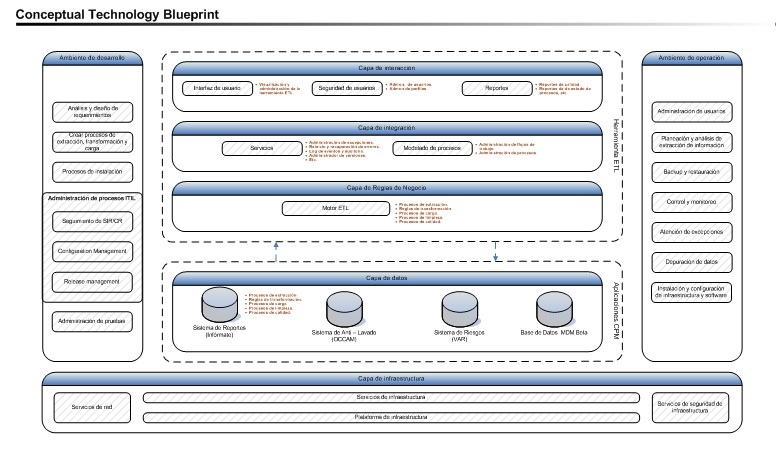
\includegraphics[width=12cm, height=4.5cm, scale=0.5]{Tecnologia_Conceptual.jpg}
        \caption{Tecnología conceptual.}
    \label{fig:conceptual}
  \end{center}
\end{figure}

\subsection{Ambiente de desarrollo}

Dentro del ambiente de desarrollo se encuentran definidas todas las actividades
que se requieren tener para la construcción de los procesos ETL, así como la
administración de los procesos y las pruebas. El ambiente de desarrollo tiene
los siguientes componentes:

\begin{itemize}

\item \textit{Análisis y diseño de requerimientos}: Dentro de la etapa de
  análisis y diseño de requerimientos encontramos la documentación de las
  fuentes y destinos de datos que serán procesadas mediante el ETL; el análisis
  de requerimientos abarca los requerimientos funcionales y técnicos que
  requiere la institución financiera para poder generar los datos en los
  sistemas destino.  Por su parte el diseño de los requerimientos incluyó el
  diseño funcional y técnico de todos los procesos a implementar dentro del ETL
  así como la definición de las reglas de programación y estándares que se
  tenían que seguir para un mejor desarrollo del proceso.

\item \textit{Creación de procesos de extracción, transformación y carga}: Una
  vez realizado el análisis y diseño de los procesos, el siguiente paso es
  construir los procesos ETL dentro de la herramienta seleccionada; para
  realizar este desarrollo se deberá de basar en el diseño funcional, en las
  reglas de transformación y en las reglas de negocio definidas dentro del
  propio diseño. El proceso de extracción para la primera iteración fue
  solamente del Core Bancario ICBS, mientras que las transformaciones y la carga
  se realizó de acuerdo al sistema al que se cargaron los datos.

\item \textit{Procesos de instalación}: Los procesos de instalación se refieren
  a los procesos a seguir para instalar el ETL dentro de los diferentes
  ambientes (desarrollo, pruebas y producción); este proceso también incluyó la
  instalación de la herramienta de ETL en la que se desarrollaron los procesos.
  Parte importante del proceso dentro del ambiente de desarrollo fue la
  administración de los procesos de ITIL, como parte de este proceso se tenía el
  seguimiento de reportes de incidencias (SIR) y controles de cambio (CR), la
  administración de configuraciones y la administración de versiones.

\item \textit{Reporte de incidencias y controles de cambio}: Se llevó a cabo un
  control de incidencias y control de cambios para todos los elementos
  desarrollados dentro del ETL.

\item \textit{Administración de configuraciones}. La administración de
  configuraciones fue parte importante dentro del ambiente de desarrollo por lo
  que fue necesario tener un registro de todas las configuraciones que se
  realizaron dentro de la herramienta.

\item \textit{Administración de versiones}. Toda herramienta ETL debe tener una
  administración de versiones para llevar el control de todos los cambios hechos
  en el desarrollo.

\item \textit{Administración de pruebas}: Como todo proyecto de implementación,
  fue necesario llevar una administración de las pruebas; las pruebas que se
  llevaron a cabo dentro de este proceso fueron: pruebas unitarias, pruebas de
  integración, pruebas de performance y pruebas de usuarios

\end{itemize}

\section{Diseño de los programas ETL}

Como parte de la herramienta ETL se integraron tres áreas que tenían relación
con los requerimientos de negocio: la capa de interacción, la capa de
integración y la capa que conteía las reglas de negocio.

\begin{itemize}

\item Capa de interacción. Esta capa se refería a la interacción que tenían
  los usuarios con la herramienta ETL; así como la explotación de todos los
  elementos de la misma. Las principales funciones que se ejecutaron dentro de
  esta capa fueron la interfaz de usuario, la administración de protocolos de
  seguridad de usuarios y los reportes.

\item Capa de integración. En esta capa hicimos referencia a todos los
  servicios y modelado de procesos necesarios para el buen funcionamiento de
  nuestra herramienta ETL. Los principales procesos que se tomaron en cuenta
  fueron los siguientes:

  \begin{itemize}
  \item \textbf{Servicios}. Servicios necesarios para el manejo de errores,
    excepciones, versiones, así como servicios adicionales necesarios para los
    procesos de extracción, transformación y carga. Tales servicios se
    dividieron en: Administración de excepciones, reinicio y recuperación de
    errores, registros de eventos y auditoria y administración de versiones.
  \item \textbf{Modelado de procesos}. Fueron principalmente los procesos
    necesarios para la creación de los programas ETL.
  \end{itemize}

\item Reglas de negocio. Dentro de este proceso definimos las reglas para la
  transformación y carga correcta de los datos en la base de datos, así como la
  funcionalidad correcta que requería la entidad financiera. La principal
  herramienta que se tuvo en esta capa, fue el motor ETL y sus principales
  tareas fueron las siguientes:

  \begin{itemize}
  \item \textbf{Procesos de extracción.} Definición de todos los procesos
    utilizados para realizar la extracción de datos
  \item \textbf{Reglas de transformación.} Definición de todas las
    transformaciones utilizadas desde la extracción de datos hasta la carga de
    los mismos en la nueva estructura de base de datos.
  \item \textbf{Proceso de carga de datos.} DEscripción de los procesos de carga
    de datos a cada uno de los sistemas destino.
  \item \textbf{Proceso de limpieza de datos.} Descripción de los procesos de
    limpieza de datos como: direcciones, teléfonos, nombres, RFCs y fechas.
  \item \textbf{Procesos de calidad.} Descripción de los procesos a seguir de
    acuerdo a los estándares de datos para tener una mejor calidad en la
    información.
  \end{itemize}

\end{itemize}

\section{Capa de datos}

La capa de datos estaba conformada por los diferentes sistemas desde donde se
extrajo la información así como los sistemas donde se almacenarían los
datos. Como sistema para extracción de datos solo se consideró un sistema,
mientras que la carga se realizó hacia tres diferentes sistemas de la
institución financiera. A continuación describo el tipo de información que se
procesaba en cada uno de los sistemas destino:

\begin{itemize}

\item Se tenía el sistema de detección de fraudes o posible mal manejo de una
  cuenta; esta detección se realizaba mediante el monitoreo de las cuentas que
  se enviaban a cada uno de los archivos generados por el procesador principal
  de transacciones bancarias.

\item El sistema de manejo de riesgos contenía la información de las cuentas
  con pagos vencidos o que presentaban algún grado de morosidad. Esta
  información también se obtenía del procesador principal de transacciones
  bancariasy sería procesada por la herramienta ETL que se implementó.

\item Finalmente, existía el sistema para el manejo de los reportes operativos
  que requería la organización. La principal tarea de este sistema era generar
  reportes regulatorios previamente definidos, así como extracción de
  información bajo demanda.
\end{itemize}

\chapter{Diseño detallado}

En este capítulo se analiza el diseño detallado, comenzando por qué tan
frecuentemente se extraen los datos y las dependencias de dichas extracciones.

\section{Dependencias y frecuencia de las extracciones de datos}

Como primer paso dentro dle proceos de extracción se identificaron las
dependencias de los sistemas origen con otros procesos, tareas o reglas de
negocio dentro de la organizción, así como la frecuencia esperada o deseada de
la extracción de datos. La extracción de datos se realizó con una periodicidad
diaria; esto debido a que al tratarse del sistema principal de la institución
financiera la información se actualizaba de manera diaria. La herramienta ETL
nos permitió identificar aquellas tablas y campos que sufrian modificaciones, de
tal forma que se extrajo solo la información que sufría cambios a lo largo del
día. La extracción de datos se realizó en un horario no operativo, a fin de no
afectar la operación de la institución; además este proceso dependía del termino
del proceso de cierre diario de operaciones. Solamente uan vez que el proceso
hubiera terminado comenzaba la extracción por parte de la herramienta ETL; este
proceso contaba con una ventana de procesamiento de 5 horas. La extracci''on fue
almacenada en la base de datos temporal dentro de la herramienta ETL.

\subsection{Extracción inicial}

En la extracción inicial se realizaron las siguientes transformaciones:

\begin{itemize}
\item Transformación de fecha jualiana a fecha gregoriana.
\item Cambio en los tipos de dato al momento de almacenarlos en la tabla
  temporal; principalmente transformación del tipo de dato \textit{char} al tipo
  de dato \textit{varchar} y los datos númericos a decimal.
\end{itemize}

Al momento de que se terminaba la extracción de datos, se cerraba la conexión a
la base de datos del procesador principal de transacciones bancarias a fin de
liberar la carga de trabajo del mismo para continuar con su operación diaria.

\subsection{Extracciones subsecuentes}

Después de realizada la extracción inicial desde el sistema fuente y con los
datos almacenados en el repositorio temporal, las siguientes extracciones se
realizaron mediante extracciones incrementales con base en la adición,
actualización o eliminación de datos de las tablas seleccionadas. Se consideró
realizar la extracción total de los registros solo en caso de que las
modificaciones o actualizaciones en la base de datos fueran muchas; las
condiciones para realizar la extraccióncompleta fueron las siguientes:

\begin{enumerate}
\item Existían cambios en más del 50\% de los registros.
\item Los registros extraídos no se encontraban actualizados o contenían
  errores.
\item Los registros extraídos no cuentan con la calidad necesaria.
\end{enumerate}

\subsection{Relación entre las entidades de datos}

En el siguiente diagrama se puede visualizar la relación entre las diferentes
entidades y los datos que comparten cada uno de ellos.

\begin{figure}[htb]
  \begin{center}
    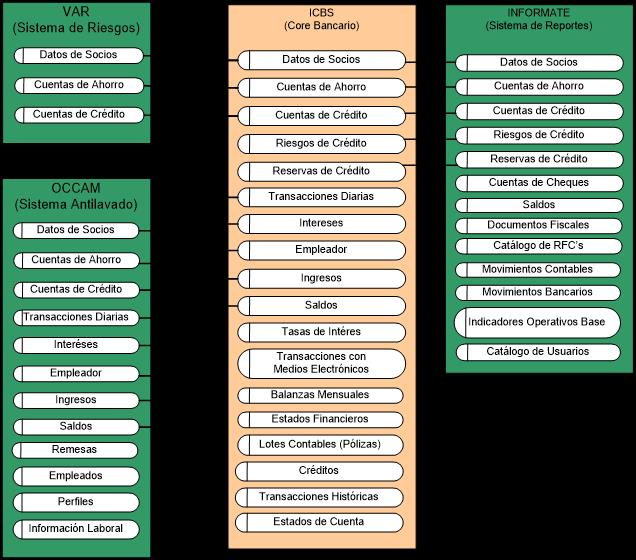
\includegraphics[width=12cm, height=3cm, scale=0.5]{Relacion_entidades.jpg}
        \caption{Datos relacionados en las entidades.}
    \label{fig:arquitectura}
  \end{center}
\end{figure}

En la imagen podemos observar que los diferentes sistemas manejan el mismo tipo
de información; socios, cuentas, créditos y saldos.

\section{Diseño para la transformación de datos}

La transformación de los datos tenía varios procesos que se deberían seguir,
entre los cuales se encuentra la limpieza de datos, los estándares y
procedimientos utilizados, así como las reglas de transformación definidas para
cada uno de los sistemas destino. La transformación de los datos se realizó
dentro de la misma base de datos de paso y se almacenó en otra instancia de esta
misma base de datos. El siguiente diagrama muestra como se realizarón las
transformaciones requeridas.

\begin{figure}[htb]
  \begin{center}
    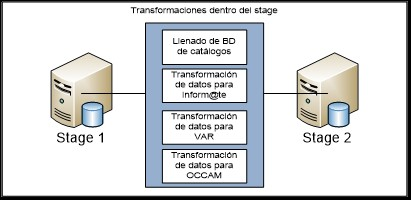
\includegraphics[width=12cm, height=3cm, scale=0.5]{Transformaciones_stage.jpg}
    \caption{Transformaciones en base de datos temporal.}
    \label{fig:arquitectura}
  \end{center}
\end{figure}

A continuación se detallan las reglas utilizadas para realizar la transfocmacón
de datos.

\subsection{Limpieza de la fuente de datos}

La limpieza de la fuente de datos \textbf{NO} estaba dentro del alcance del
proyecto; sin embargo se realizaron las transformaciones de la fuente de datos
para realizar la limpieza de datos hacia los sistemas destino. Como parte de un
proceso de calidad de la información y limpieza de datos se definierón los
siguientes criterios:

\begin{enumerate}

\item Los nombres de los socios debían contener solamente caracteres
  alfabéticos; no se permitieron caracteres especiales como los siguientes:
  ``\textbackslash'', ``.'', ``\#'', ``\$'', ``\%'', ``\&''.

\item Los números telefónicos debían contener solamente caracteres numéricos y
  debían ser de 10 posisciones para teléfonos fijos y 13 posiciones para
  teléfonos celulares.

  \begin{itemize}
  \item Si \textit{Tipo\_Telefono} $=$ Casa y Longitud $($Telefono$)$ $=$10
    Entonces Telefono\_Casa SiNo Error
  \item Si \textit{Celular} $=$ Casa y Longitud $($Telefono$)$ $=$ 13 Entonces
    Telefono\_Celular SiNo Error
  \end{itemize}

\item El RFC de los socios debería ser de 10 o 13 posiciones para las personas
  físicas y 12 posiciones para las personas morales. En caso de no contar con un
  RFC valido, el registro era rechazado y enviado a una tabla de auditoria para
  su corrección dentro del sistema fuente de parte del área de tecnología de la
  compañia.

\item Todos los códigos postales debían ser de cinco dígitos, en caso de existir
  algún registro con mayor o menor número, estos debían de ser enviados a una
  tabla de auditoria para su corrección dentro del sistema fuente. Se consideró
  una homologación de datos para los códigos de ciudades y estados. Todos los
  códigos de estados se homologaron a tres dígitos que corresponden a las tres
  primeras letras de cada estado; se realizó unaexcepción para el caso de
  Chiapas (CHS) que podría confundirse con Chihuahua (CHI).

\item Las fechas se homologaron al formato yyyymmdd y no debían permitir valores
  nulos o fechas inválidas.

\end{enumerate}

\subsection{Estándares y procedimientos utilizados para la interrelación de los datos}

Para realizar una estandarización de los datos se creó una base de datos
temporal que conternía la información de todos los campos con los mismos datos
pero que su sistema origen era diferente. La creación de esta tabla temporal fue
crear la base para generar una tabla de referencias cruzadas que representara un
gobierno de datos o MDM (Master Data Management) por sus siglas en Inglés

\subsection{Reglas utilizadas para la transformación de datos}

Como regla general para todos los procesos de extracción se realizaron las
siguientes transformaciones.

\begin{itemize}
\item Transformación de fechas julianas a fechas gregorianas en formato
  \linebreak \mbox{yyyy/mm/dd}.
\item Transformación de los tipos de dato origen a los tipos de la base de
  datos stage generada en SQL Server.
\end{itemize}

Los procesos de transformación para cada destino fueron diferentes debido a las
características de cada uno de los archivos de salida. Dichas transformaciones
se realizaron tomando como principal fuente de datos, la base de datos temporal.

\subsubsection{Sistema de reportes}

\begin{itemize}

\item Todos los campos de fecha que tengan un sufijo \_d deberían de ser
  convertidas a formato de fecha $($yyyymmdd$)$ para todas las tablas de este
  sistema. Se pobló la fecha de vencimiento \_D, tomando como base el campo
  fecha de vencimiento de la tabla de facturación. La regla de transformación
  que se definió fue la siguiente:

\begin{verbatim}
FEC_VENCIMIENTO_5_D = CAST(RIGHT(LTRIM(RTRIM(FEC_VENCIMIENTO_5)),2) +
        LEFT(RIGHT(LTRIM(RTRIM(FEC_VENCIMIENTO_5)),4), 2) +
        REPLICATE('0', 2-len(LEFT(LTRIM(RTRIM(FEC_VENCIMIENTO_5)),
        ABS(4-len(LTRIM(RTRIM(FEC_VENCIMIENTO_5))))))) +
        LEFT(LTRIM(RTRIM(FEC_VENCIMIENTO_5)),
        ABS(4-len(LTRIM(RTRIM(FEC_VENCIMIENTO_5))))) AS DATETIME)
        WHERE  FEC_VENCIMIENTO_5 > 0
\end{verbatim}

\item Para el campo Fecha de último saldo se tomó la fecha de vencimiento más
  antigua que se tenía.
\item Para obtener el número de créditos de un socio se realizó la siguiente
  regla.

\begin{verbatim}
        NO_CREDITOS =  NO_CREDITOS
        WHERE  NO_SOCIO IN NO_SOCIO de la tabla CIF_CREDITOS.
        Si NO_CREDITOS = NULL Entonces NO_CREDITOS = 0
\end{verbatim}

\item La descripción de la información correspondiente a las garantías debía
  de estar vacio en la tabla destino.

\item Para almacenar la fecha de último monto con saldo se tomó la fecha de
  vencimiento más antigua que se tenía para cada registro dentro de la tabla de
  saldos \textit{LN\_SALDOS.}

\item Se realizó una validación sobre el tipo de cuenta para confirmar su
  valor $=$ 1 $($Personas físicas$)$ o 6; en estos casos se colocó un valor 20
  dentro del campo Tipo\_producto de la tabla TA\_SALDOS.

\item El número de docio para poblar la tabla TA\_SALDOS se obtuvo de la
  tabla de cuentas por socio, pero solamente de aquellas cuentas cuyo tipo de
  producto era 4 u 8 y que tuvieran un saldo en la tabla TA\_SALDOS.

\item Se calculó el número de créditos de cada socio y este valor se grabó en
  la tabla CIF\_INFGEN; en caso de que el número de créditos fuera nulo se
  colocó un valor por default 0.

\item Se insertó el número de socio dentro de la tabla TA\_CTAXSOCIO para
  aquellos números de cuenta menores a 20000000000 y cuya clave de relación
  fuera 'SOW' u 'OWN'. El número de socio eran los 10 dígitos de la derecha de
  cada número de cuenta.

\item Se definió que para el campo descripción perteneciente a la tabla
  LN\_GARANTIAS debería poblarse con un valor NULL a pesar de tener mapeado un
  campo del cuál se extraía la información.

\item El campo Periodo de la tabla LN\_SALDOS se asignó con un valor fijo =
  'M'.

\item El campo frecuencia de la tabla LN\_SALDOS se asignó con un valor fijo
  $=$ 30.

\end{itemize}

La regla de transformación que se utilizó durante la extracción.

\subsubsection{Reglas para el sistema para prevención de lavado de dinero}

Las reglas definidas para este sistema son las siguientes:

\begin{itemize}
\item Se definieron algunos valores estáticos para los tres primeros campos de
  cada uno de los archivos generados; estos valores son los siguientes:
\begin{enumerate}
\item Valor fijo 'CMPS' para el primer campo.
\item Valor fijo 'T' para el segundo campo.
\item Valor fijo 'F' para el tercer campo.
\end{enumerate}
\item Para la generación del archivo de cuentas se tomaron solo aquellas
  cuentas que tuvieron movimientos durante el día.
\item Solamente se tomaron en cuenta los siguientes tipos de cuenta: Parte
  social, cuenta mexicana, servicuenta y cuentamiga.
\item Si el tipo CIF es una persona moral (CUTYP $=$ 5), entonces el campo
  CompanyLegalId se pobló con dicho valor, en caso contrario se asignó un valor
  constante vacio ``''.
\end{itemize}

\section{Arquitectura aplicativa}

% TODO

\section{Arquitectura de negocio}

% TODO

\section{Arquitectura de datos}

Como se explicó en los capitulos anteriores, la institución financiera contaba
con diferentes procesos ETL que extraían información del sistema
principal. Estos sistemas trabajaban de manera independiente por lo que cada
sistema destino tenía su base de datos temporal antes de enviarla a su
destino. La arquitectura se encuentra detallada en el siguiente diagrama:

\begin{figure}[htb]
  \begin{center}
    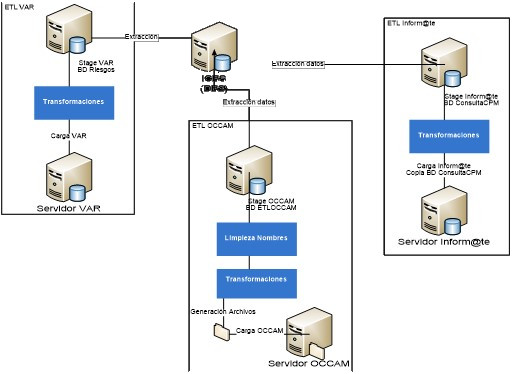
\includegraphics[width=12cm, height=3cm, scale=0.5]{Arquitecturadatos_actual.jpg}
    \caption{Arquitectura de datos actual.}
    \label{fig:arquitecturaactual}
  \end{center}
\end{figure}

Como se observa en la imagen anterior, existían muchas bases de datos
intermedias entre la fuente de datos y los sistemas destino; la arquitectura
definida dentro de este proyecto, nos permite tener una sola base de datos
temporal, así como una sola capa de integración de datos. El siguiente diagrama
muestra el diseño de la arquitectura desarrollada:

\begin{figure}[htb]
  \begin{center}
    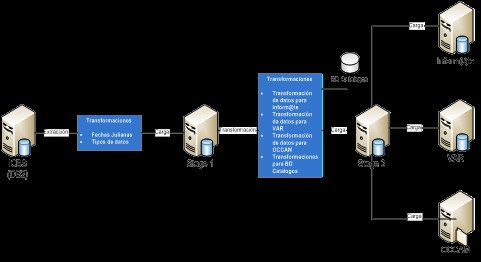
\includegraphics[width=12cm, height=3cm, scale=0.5]{Arquitectura_final.jpg}
    \caption{Arquitectura de datos actual.}
    \label{fig:Arquitecturafinal}
  \end{center}
\end{figure}

Arquitectura\_final % ???

\section{Arquitectura de infraestructura}

``Diseño de arquitectura aplicativa'', ``Arquitectura de negocio'',
``Arquitectura de datos'' y ``Arquitectura de infraestructura''

\chapter*{Modelo de datos}

% si no queremos que añada la palabra ``Capitulo''
\label{cap.modelo}
% si queremos que aparezca en el índice
\addcontentsline{toc}{section}{Modelo de datos}
% encabezado
\markboth{Modelo de datos}{Modelo de datos}

\section{Modelo de datos lógico}

\section{Modelo de datos físico}

% si no queremos que añada la palabra ``Capitulo''
\chapter*{Estándares de programación}
% si queremos que aparezca en el índice
\label{cap.estandares}
\addcontentsline{toc}{section}{Estándares de programación}
% encabezado
\markboth{Estándares de programación}{Estándares de programación}

dalsdkla % ???

% si no queremos que añada la palabra ``Capitulo''
\chapter*{Conclusiones}
\label{cap.conclusiones}
% si queremos que aparezca en el índice
\addcontentsline{toc}{section}{Conclusiones}
% encabezado
\markboth{Conclusiones}{Conclusiones}

\end{document}
